%%==================================================
%% chapter03.tex for BIT Master Thesis
%% modified by yang yating
%% version: 0.1
%% last update: Dec 25th, 2016

%% modified by Meng Chao
%% version: 0.2
%% last update: May 29th, 2017
%%==================================================
\chapter{单目SLAM算法研究}
\label{chap:ALGORITHM}

%3.1
%\section{引言}
同步定位与地图重建算法利用多视图几何原理\upcite{[]},根据获取的图像信息估计摄像头在陌生环境中的位姿,构建环境地图。如果获取图像信息时,仅使用一个摄像头,则称为单目SLAM。本章主要介绍经典视觉SLAM算法框架;研究基于该框架的两种主流单目SLAM算法,在相同数据集上对比分析两种算法的优缺点,结合无人机运动特性选择合适的SLAM算法。

%3.1
\section{经典视觉SLAM算法框架}
SLAM算法实际是状态估计问题,将传感器数据抽象为适于估计的数学模型,通过观测模型与运动模型估计系统状态。经典视觉SLAM算法框架一般包括3个部分:视觉里程计,后端优化和闭环检测。视觉里程计估计帧间运动和局部地图,把传感器数据抽象为适于估计的数学模型;后端优化则接收视觉里程计估计的不同时刻位姿和回环检测信息,根据观测模型和运动模型建立约束关系,估计优化相机位姿与地图点位置,得到全局一致的轨迹与地图;回环检测判断相机是否曾经到达过当前位置,如果检测到回环反馈则给后端进行优化处理。算法框架如图\ref{fig3.1}所示,经典的视觉SLAM算法框架是过去十几年研究者们总结的成果,框架本身和所包含的算法已经较为成熟。本文研究内容主要是在该框架的基础上,针对单目SLAM算法存在的问题进行改进和完善。
%图3.1 高翔论文图1.3
\begin{figure}[h]
\centering
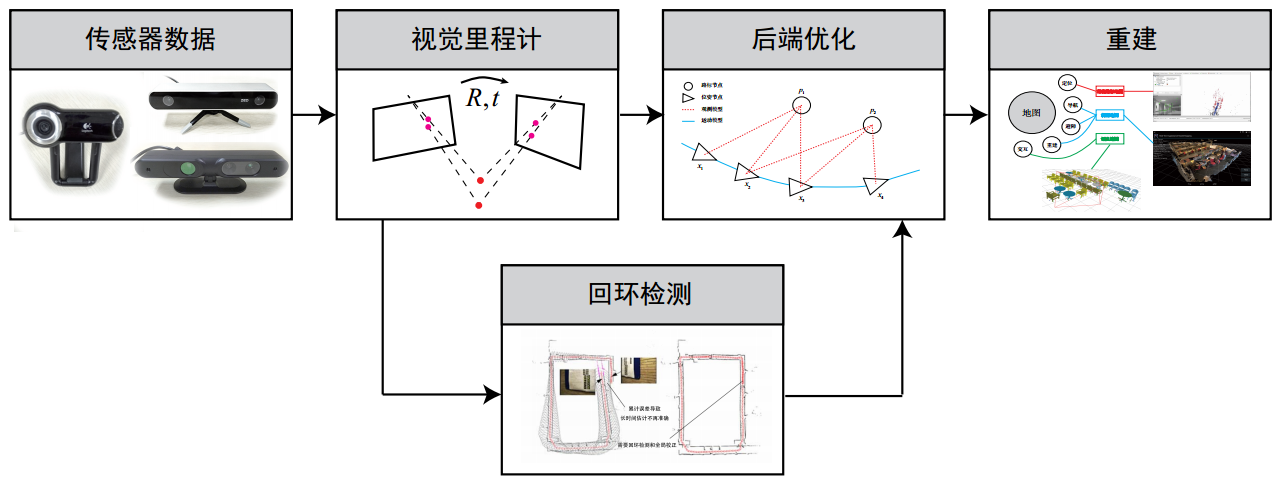
\includegraphics[scale=0.3]{figures/Fig3.1.png}
\caption{视觉SLAM算法框架}
\label{fig3.1}
\end{figure}

%3.1.1
\subsection{视觉里程计}
SLAM是一个状态估计问题,然而实际的传感器输出大都很难直接作为状态估计模型的输入。因而视觉里程计的主要任务是根据传感器输入,估计图像$I_i \rightarrow I_j$的相对位姿$T_ij$,串联相对位姿并三角化观测到的地图点得到运动轨迹与局部地图,将图像数据抽象为适于估计的数学模型。视觉里程计一般只估计相邻时刻的运动,和再过往的状态没有关联。视觉里程计主要包括两个部分,传感器数据关联和运动估计,其算法流程如图\ref{fig3.2}所示。根据视觉里程计传感器关联数据方式的不同,当前主流SLAM算法分为基于直接法和基于特征的SLAM算法,具体原理将在3.2节中详细介绍。
%图3.2 vo综述中的vo流程。
\begin{figure}[h]
\centering
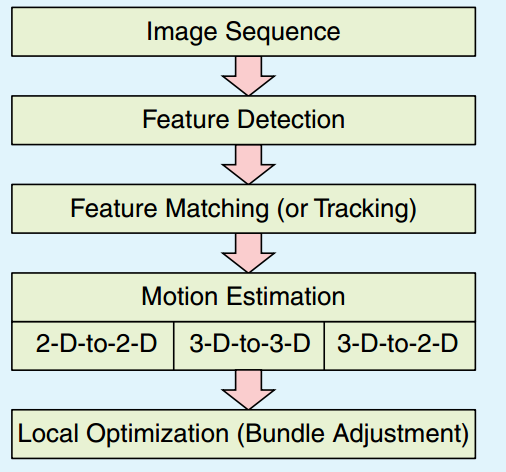
\includegraphics[scale=0.5]{figures/Fig3.2.png}
\caption{视觉里程计算法流程图}
\label{fig3.2}
\end{figure}

视觉里程计得到的轨迹和地图,由于在运动估计时只考虑了帧间的信息,每次估计都带有一定的误差,串联的轨迹无可避免会出现累计漂移,这将导致无法得到全局一致的轨迹与地图。需要通过后端优化算法进行处理,估计运动和周围环境空间的不确定性,减小估计误差,提高轨迹和地图的一致性。


%3.1.2
\subsection{后端优化}
SLAM算法的后端优化将SLAM问题看作最大后验概率估计问题,且大都采用因子图的方式来推到变量之间的以来关系。一般的,假设代估计状态变量为$\mathcal{X}$,在SLAM中变量$\mathcal{X}$包括无人机的轨迹和地图点的位置。传感器可以获得一组测量值$Z=\lbrace z_k:k=1,\ldots ,m\rbrace$,且每个测量值可以表示为状态变量$\chi$的函数,例如$z_k=h_k\left( \mathcal{X}_k \right)+\epsilon_k$,其中$\mathcal{X}_k \in \mathcal{X}$是变量的子集,$h_k(\cdot)$表示传感器的观测模型,$\epsilon_k$是随机观测误差。

在最大后验概率估计中,通过计算变量$\mathcal{X}^*$的概率分布来估计状态变量$\mathcal{X}$,$\mathcal{X}^*$表示最大后验概率$\mathds{P}\left(\mathcal{X} \vert Z\right)$:
\begin{equation}
\label{equ3.1}
\mathcal{X}^* 
\doteq 
\argmax \limits_{\mathcal{X}} \mathds{P}\left(\mathcal{X} \vert Z\right) 
=
\argmax \limits_{\mathcal{X}}\mathds{P}\left(Z \vert \mathcal{X}  \right)\mathds{P}\left(\mathcal{X}\right)
\end{equation}
上式推导来源于贝叶斯定义。在公式\eqref{equ3.1}中,$\mathds{P}\left(Z \vert \mathcal{X}  \right)$表示在状态变量$\mathcal{X}$分布确定情况下测量值$Z$的似然,$\mathds{P}\left(\mathcal{X}\right)$表示状态$\mathcal{X}$的先验概率。先验概率包括任何关于状态$\mathcal{X}$的先验信息,如果没有可用的先验信息,则$\mathds{P}\left(\mathcal{X}\right)$表示为一个常亮从而可以从优化过程中移除。在这种情况下,最大后验概率可以简化为极大似然估计。

假设测量值$Z=\lbrace z_k:k=1,\ldots ,m\rbrace$相互独立(影响测量的噪声是不相关的),公式\eqref{equ3.1}可以因式分解为:
\begin{equation}
\label{equ3.2}
\mathcal{X}^* 
\doteq 
\argmax \limits_{\mathcal{X}} \mathds{P}\left(\mathcal{X}\right) \prod \limits_{k=1}^{m} \mathds{P}\left(z_k \vert \mathcal{X}  \right)
=
\mathds{P}\left(\mathcal{X}\right) \prod \limits_{k=1}^{m} \mathds{P}\left(z_k \vert \mathcal{X}_k  \right)
\end{equation}
其中,等式右边的测量值$z_k$仅仅与状态变量$\mathcal{X}_k$的子集有关。

公式\eqref{equ3.2}可以因子图表示。待估计的状态变量用节点表示,似然$\mathds{P}\left(z_k \vert \mathcal{X}_k  \right)$和先验$\mathds{P}\left(\mathcal{X} \right)$由因子表示,因子建立了对节点子集的概率约束。因子图是一种建立第$k$个因子和对应状态变量$\mathcal{X}_k$依赖关系的图模型。因子图可以将SLAM问题可视化,便于理解,SLAM算法的因子图描述如图\ref{fig3.3}表示。
% 综述因子图
\begin{figure}
\centering
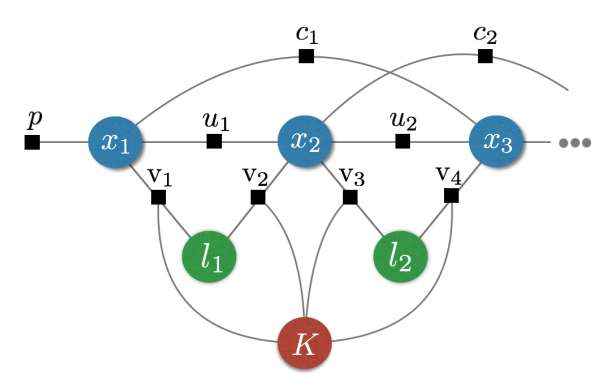
\includegraphics[scale=0.5]{figures/Fig3.3.png}
\caption{SLAM因子图}
\label{fig3.3}
\end{figure}


为了更清楚的表示公式\eqref{equ3.2},假设观测模型的测量噪声$\epsilon_k$服从信息矩阵为$\Omega_k$的0均值高斯分布。测量值的似然可以表示为
\begin{equation}
\label{equ3.3}
\mathds{P}\left(z_k \vert \mathcal{X}_k  \right) \varpropto \exp ( -{1 \over 2} \left\| h_k\left( \mathcal{X}_k \right) - z_k \right\|_{\Omega_k}^2 )
\end{equation}
其中,使用符号$\left\| e \right\|_{\Omega}^2 = e^T \Omega e$。类似的,假设先验也服从高斯分布:
\begin{equation}
\label{equ3.4}
\mathds{P}\left( \mathcal{X}_k  \right) \varpropto \exp ( -{1 \over 2} \left\| h_0\left( \mathcal{X}_0 \right) - z_0 \right\|_{\Omega_0}^2 )
\end{equation}
其中$h_0(\cdot)$表示观测模型,先验均值为$z_0$,信息矩阵为$\Omega_0$。由于最大后验与最小负对数后验等价,则公式\eqref{equ3.2}的最大后验估计可以表示为:
\begin{equation}
\label{equ3.5}
\mathcal{X}^* 
=
\argmin \limits_{\mathcal{X}} - \log \left( \mathds{P}\left(\mathcal{X}\right) \prod \limits_{k=1}^{m} \mathds{P}\left(z_k \vert \mathcal{X}_k  \right) \right)
=
\argmin \limits_{\mathcal{X}} \sum \limits_{k=0}^{m} -{1 \over 2} \left\| h_k\left( \mathcal{X}_k \right) - z_k \right\|_{\Omega_k}^2
\end{equation}
公式\eqref{equ3.5}的形式是典型的非线性最小二乘问题,其中$h_k{\cdot}$是一个非线性函数。需要注意的是,公式\eqref{equ3.5}推导的前提是假设观测模型的观测噪声服从高斯分布。对于不同的观测噪声分布,将会得到不同的优化目标函数。例如,若观测噪声服从拉普拉斯分布,则公式\eqref{equ3.5}的平方$l_2$范数应变为$l_1$范数。为了增加算法对于离群点的鲁棒性,通常使用鲁棒核函数替换公式\eqref{equ3.5}中的平方$l_2$范数。

公式\eqref{equ3.5}的形式与运动结构学中的Bundle Adjustment(BA)问题相似。这是因为公式\eqref{equ3.5}与BA都是从最大后验概率估计出发推导得到的。但是,SLAM问题具有两个特点。首先,不同于BA问题受限于几何模型约束,公式\eqref{equ3.5}适用于各种传感器模型。比如惯性传感器,GPS,轮式传感器等。其次,公式\eqref{equ3.5}是增量式的求解,在无人机运动时,可以获得新的观测值。

对于解决公式\eqref{equ3.5}的最小化问题,可通过连续线性化进行求解。例如高斯-牛顿法(G-N)和列文伯格-马夸尔特法(L-M)。高斯-牛顿方法从初始估计给定的初值$\hat{\mathcal{X}}$开始迭代,每次迭代时高斯-牛顿法估计公式\eqref{equ3.5}的最小值
\begin{equation}
\label{equ3.6}
\delta_\mathcal{X}^* 
=
\argmin \limits_{\delta_\mathcal{X}} {1 \over 2} \sum \limits_{k=0}^{m} \left\| A_k\delta_\mathcal{X}-b_k \right\|_{\Omega_k}^2
=
\argmin \limits_{\delta_\mathcal{X}} {1 \over 2} \left\| A_k\delta_\mathcal{X}-b \right\|_{\Omega}^2
\end{equation}
其中公式\eqref{equ3.6}中的$\delta_\mathcal{X}$表示初始估计状态$\hat{\mathcal{X}}$的微小修正量。$A_k \doteq {\partial h_k(\mathcal{X}) \over \partial \mathcal{X}} $是观测模型$h_k(\cdot)$关于$\mathcal{X}$的雅各比,$b_k \doteq z_k-h(\mathcal{X})$表示测量值与观测模型输出的残差;公式\eqref{equ3.6}右边的矩阵$A$,$b$是由$A_k$,$b_k$组成的矩阵;$\Omega$是由观测噪声信息矩阵$\Omega_k$组成的对角块矩阵。

最小化公式\eqref{equ3.6}对应的微小修正$\delta_\mathcal{X}^* $可以用下面的闭型公式计算
\begin{equation}
\label{equ3.7}
\delta_\mathcal{X}^* = - \left( A^T \Omega A \right)^{-1} A^T \Omega b
\end{equation}
每次通过$\hat{\mathcal{X}} \leftarrow \hat{\mathcal{X}}+\delta_\mathcal{X}^*$迭代更新估计状态,矩阵$A^T \Omega A$称为Hessian矩阵。之前的推导过程中,我们假设$\mathcal{X}$属于向量空间。如果$\mathcal{X}$属于光滑的流形空间(如旋转),则高斯-牛顿法的形式保持不边,但是迭代更新方程$\hat{\mathcal{X}} \leftarrow \hat{\mathcal{X}}+\delta_\mathcal{X}$会被更合适的映射法则取代。在机器人领域中,通常使用符号$\oplus$表示状态更新的映射关系,并且将状态的微小修正量$\delta_\mathcal{X}$定义在流形状态变量$\hat{\mathcal{X}}$的切空间上,此时的更新方程为$\hat{\mathcal{X}}  \leftarrow \hat{\mathcal{X}} \oplus \delta_\mathcal{X}$。

现代SLAM算法最大的进步,在于认识到公式\eqref{equ3.7}中的雅各比矩阵$A$的稀疏性,而矩阵$A$的稀疏性是由于因子图内在的拓扑逻辑所决定的,这可以利用线性方法快速求解估计状态的微小增量$\delta_\mathcal{X}^*$。此外,利用矩阵$A$的稀疏性可以设计增量式的求解方法,将更新后的状态变量作为新的观测值。当前主流SLAM后端优化库(如GTSAM,g2o,Ceres,iSAM,SLAM++)可以在几秒之内求解数以万计的状态变量。

目前,通常使用最大后验估计,因子图优化,图优化,完全平滑和平滑映射来描述SLAM问题。其中特别需要介绍的描述方法是位姿图优化,位姿图中的状态变量是无人机运动中的采样位姿,约束是两位姿之间的相对运动约束。

%3.1.3
\subsection{回环检测}
前两节介绍了前端视觉里程计和后端优化:前端将传感器观测到的数据进行关联并将数据抽象为适于后端估计的数据(轨迹,地图点位置);后端负责根据前端的结果对系统状态进行优化。然而,前端的视觉里程计只考虑时间关联性,之前测量产生的误差不可避免的会累计到下一时刻,使得SLAM出现累计误差,无法构建权全局一致的轨迹和地图。后端优化虽然能够估计最大后验误差,但由于前端只提供了相邻时刻关键帧数据,无法消除累计误差。回环检测又称闭环检测,负责检测传感器是否经过同一个位置,通过增加窗时间下的数据关联性约束,消除SLAM的轨迹与地图随时间漂移而产生的累计误差。回环检测对于SLAM算法意义重大,关系到SLAM算法估计的轨迹和地图在长时间下的准确性。另外,由于回环检测可以提供当前数据与历史数据的关联性,当SLAM算法前端跟踪失效丢失后,可以利用回环检测进行重定位,有效提高整个SLAM算法的精度和鲁棒性。

常用的回环检测方法有两种:基于里程计的几何关系或基于外观的图像间相似性。基于里程计的几何方法利用视觉里程计的位置信息,当发现运动到之前的某个位置附近时检测是否有回环关系。这是一种很直接的检测思路,但是由于存在累计误差,里程计无法正确的发现到是否回到了曾经的某个位置。另一种方法是基于外观的,这种方法和前端后端的输出都无关,仅仅根据两幅图像之间的相似性进行判断。这种方法与累计误差完全无关,可以独立作为SLAM算法的一个模块,成为视觉SLAM中的主流算法,应用与多个实际的系统中。


%3.2
\section{主流单目视觉SLAM算法研究}
近些年出现了许多优秀的单目SLAM算法理论,按照前端视觉里程计关联数据的方式不同主要分为基于直接法的SLAM算法和基于特征的SLAM算法两种。基于直接法SLAM算法假设同一空间点的像素灰度值在不同图像中固定不变,估计最优位姿使得两幅图像经变换后灰度变化最小,完成前端的数据关联。基于特征的SLAM算法则提取图像中的特征,并在不同图像间对相同特征进行匹配,从而解算图像之间的相对运动,关联前端数据。本节主要研究两种具有代表性的单目SLAM算法:LSD-SLAM和ORB-SLAM。分析两算法的原理、优势和不足,针对单目SLAM算法存在的不足提出改进方向。

%3.2.1
\subsection{基于直接法的LSD-SLAM}


\subsubsection*{算法概述}
LSD-SLAM是2014年慕尼黑工业大学的J.Engle等人提出的基于直接法的SLAM算法,无需计算图像特征点,通过直接法的像素关联估计运动状态,构建半稠密地图——这里的半稠密是指估计灰度梯度明显区域的像素位置。该算法可以在大尺度环境下实时运行,利用半稠密像素关联和关键帧pose图构建全局一致的地图,关键帧间的约束pose图使用相似变换$\mathfrak{sim}(3)$代替$\mathfrak{se}(3)$显示的表示尺度,从而在后端优化中可以考虑不同场景的尺度,减小尺度漂移。LSD-SLAM算法的流程如图\ref{fig3.4}所示
%LSD算法流程图
\begin{figure}
\centering
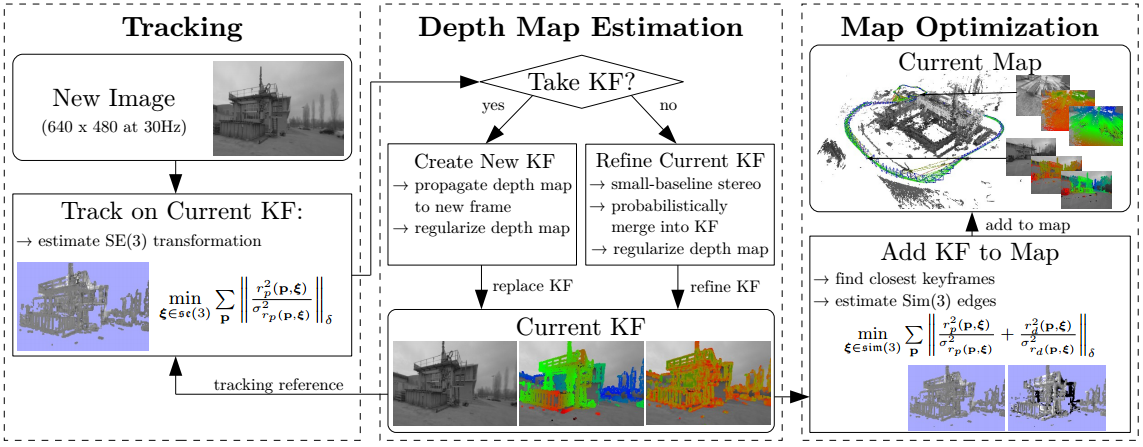
\includegraphics[scale=0.35]{figures/Fig3.4.png}
\caption{LSD-SLAM算法流程图\upcite{}}
\label{fig3.4}
\end{figure}

LSD-SLAM算法主要分为三个模块:图像跟踪,地图深度估计和地图优化。图像跟踪模块获取传相机采集的图像,利用上一帧的图像位姿作为初值,估计当前帧相对于关键帧的相对位姿$\xi \in \mathfrak{se}(3) $;地图深度估计模块根据前帧情况,进行关键帧替换或优化当前关键帧的位姿和地图点深度。如果相机运动过快,则将新关键帧的地图点投影到临近关键帧进行初始化;如果当前帧被创建为新的关键帧,则之前的关键帧的深度不再被优化。地图优化模块将之前的关键帧加入到全局地图中,使用尺度感知和相似变换图像关联来检测回环和尺度漂移,估计相邻关键帧之间的相似变换$\xi \in \mathfrak{sim}(3)$优化关键帧的位姿和深度。

\subsubsection*{数据关联与运动估计}
基于直接法的SLAM算法的前提是灰度不变假设,即认为同一空间点的像素灰度值,在不同图像中保持不变。直接法预先不知道单个像素与像素间的对应关系,而是通过最小化光度误差来求解位姿变换和对应关系。如图\ref{fig3.5}所示,空间某点P和两时刻图像上的对应像素点。空间点P的世界坐标为$[X,Y,Z]^T$,内参为$\boldsymbol{K}$的两相机对应的像素坐标为$\boldsymbol{p_1},\boldsymbol{p_2}$。为了估计从相机1到相机2的相对位姿,以相机1为参考系假设相机2的位姿为$\boldsymbol{R},\boldsymbol{t}$,对应的李代数为$\boldsymbol{\xi}$。根据相机投影模型有:
\begin{equation}
\label{equ3.8}
\begin{aligned}
& \boldsymbol{p_1} = 
\begin{bmatrix}
u_1 \cr v_1 \cr 1 \cr 
\end{bmatrix}
={1 \over Z_1} \boldsymbol{K} \boldsymbol{P}
\\
& \boldsymbol{p_2} = 
\begin{bmatrix}
u_2 \cr v_2 \cr 1 \cr
\end{bmatrix}
={1 \over Z_2} \boldsymbol{K} ( \boldsymbol{R} \boldsymbol{P}+\boldsymbol{t}) = {1 \over Z_2} \boldsymbol{K} ( \exp (\boldsymbol{\xi}^{\wedge}) \boldsymbol{P})_{1:3}
\end{aligned}
\end{equation}
其中$Z_1$,$Z_2$是空间点P在两个相机坐标系下的深度,$(\cdot)^{\wedge}$表示向量的反对称矩阵。由于位姿$\exp(\boldsymbol{\xi}^{\wedge})$应该与齐次坐标相乘,得到的结果只取前三个元素。
\begin{figure}
\centering
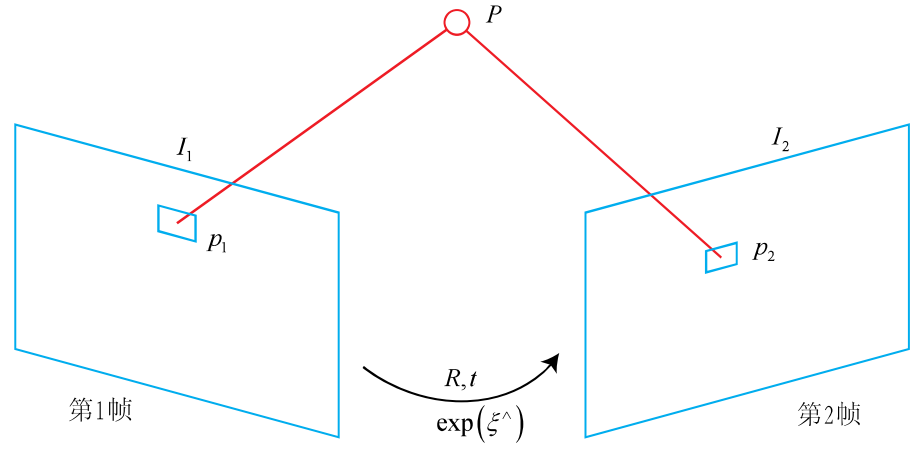
\includegraphics[scale=0.5]{figures/Fig3.5.png}
\caption{直接法示意图}
\label{fig3.5}
\end{figure}

直接法中只已知像素的灰度值,无法直接提供两幅图像的像素匹配,而是根据灰度不变假设估计相机间的相对位姿,最小化两幅图像像素之间的光度误差,也就是$P$点对应两个像素点的灰度误差。
\begin{equation}
\label{equ3.9}
\begin{aligned}
& e = I_1(\boldsymbol{p}_1) - I_2(\boldsymbol{p}_2) 
\\ 
& \min\limits_{\boldsymbol{\xi}} J(\boldsymbol{\xi}) = \Vert e \Vert ^2
\end{aligned}
\end{equation}
其中$I(\cdot)$表示图像像素灰度函数,目标优化函数为误差的二范数。对于空间中所有空间点,都应该满足灰度不变假设。若存在$N$个空间点$P_i$,则相机位姿估计问题可以表示为
\begin{equation}
\label{equ3.10}
\min\limits_{\boldsymbol{\xi}} J(\boldsymbol{\xi}) = \sum\limits_{i=1}^N e_i^T e_i
\end{equation}
其中优化函数的优化变量是相机位姿$\boldsymbol{\xi}$,为了求解最优解需要研究位姿$\boldsymbol{\xi}$变化对误差$e$的影响,即误差关于位姿的导数。使用李代数左乘扰动模型给$\exp(\boldsymbol{\xi}^{\wedge})$增加扰动$\exp( \delta \boldsymbol{\xi}^{\wedge})$,有
\begin{equation}
\label{equ3.11}
\begin{aligned}
e(\boldsymbol{\xi}\oplus \delta \boldsymbol{\xi}) & = I_1\left({1 \over Z_1} \boldsymbol{K} \boldsymbol{P} \right) - I_2\left({1 \over Z_2} \boldsymbol{K} \exp (\delta \boldsymbol{\xi}^{\wedge}) \exp (\boldsymbol{\xi}^{\wedge}) \boldsymbol{P} \right)
\\
& \simeq I_1\left( {1 \over Z_1} \boldsymbol{K} \boldsymbol{P} \right) - I_2 \left( {1 \over Z_2} \boldsymbol{K} (1+\delta \boldsymbol{\xi}^{\wedge}) \exp (\boldsymbol{\xi}^{\wedge}) \boldsymbol{P} \right)
\\
& = I_1\left( {1 \over Z_1} \boldsymbol{K} \boldsymbol{P} \right) - I_2 \left({1 \over Z_2} \boldsymbol{K} \exp (\boldsymbol{\xi}^{\wedge}) \boldsymbol{P}+ {1 \over Z_2} \boldsymbol{K} \delta \boldsymbol{\xi}^{\wedge} \exp (\boldsymbol{\xi}^{\wedge}) \boldsymbol{P} \right)
\end{aligned}
\end{equation}
记公式\eqref{equ3.11}中的$\boldsymbol{q} = \delta \boldsymbol{\xi}^{\wedge} \exp (\boldsymbol{\xi}^{\wedge}) \boldsymbol{P} $,$\boldsymbol{u}={1 \over Z_1} \boldsymbol{K} \boldsymbol{P}$,$\boldsymbol{q}$为P点在扰动下的相机2坐标系下的坐标,$\boldsymbol{u}$为它的像素坐标。利用一阶泰勒近似,有
\begin{equation}
\label{equ3.12}
\begin{aligned}
e(\boldsymbol{\xi}\oplus \delta \boldsymbol{\xi}) &= I_1\left({1 \over Z_1} \boldsymbol{K} \boldsymbol{P} \right) - I_2 \left({1 \over Z_2} \boldsymbol{K} \exp (\boldsymbol{\xi}^{\wedge}) \boldsymbol{P}+ \boldsymbol{u} \right) 
\\ 
& \simeq I_1\left({1 \over Z_1} \boldsymbol{K} \boldsymbol{P} \right) - I_2 \left({1 \over Z_2} \boldsymbol{K} \exp (\boldsymbol{\xi}^{\wedge}) \boldsymbol{P} \right) - {\partial I_2 \over \partial \boldsymbol{u}} {\partial \boldsymbol{u} \over \partial \boldsymbol{q}} {\partial \boldsymbol{q} \over \partial \delta \boldsymbol{\xi}} \delta \boldsymbol{\xi}
\\
& = e(\boldsymbol{\xi}) - {\partial I_2 \over \partial \boldsymbol{u}} {\partial \boldsymbol{u} \over \partial \boldsymbol{q}} {\partial \boldsymbol{q} \over \partial \delta \boldsymbol{\xi}} \delta \boldsymbol{\xi}
\end{aligned}
\end{equation}
在公式\eqref{equ3.12}中一阶泰勒展开的导数由链式法则分解为三项,$\partial I_2 / \partial \boldsymbol{u}$表示相机2图像中像素$\boldsymbol{u}$处的灰度梯度;$\partial \boldsymbol{u} / \partial \boldsymbol{q}$表示
相机投影方程关于相机坐标系2下的三维点的导数,假设$\boldsymbol{q} = \left[X_2,Y_2,Z_2 \right]^T$,导数为
\begin{equation}
\label{equ3.13}
{ \partial \boldsymbol{u} / \partial \boldsymbol{q} } = 
\begin{bmatrix}
\partial u \over \partial X_2 & \partial u \over \partial Y_2 & \partial u \over \partial Z_2 \cr
\partial v \over \partial X_2 & \partial v \over \partial Y_2 & \partial v \over \partial Z_2 \cr
\end{bmatrix} = 
\begin{bmatrix}
f_x \over Z_2 & 0 & -f_x X_2 \over Z_2^2 \cr
0 & f_y \over Z_2 & - f_y Y_2 \over Z_2^2 \cr
\end{bmatrix}
\end{equation}
${\partial \boldsymbol{q} \over \partial \delta \boldsymbol{\xi}}$表示相机2坐标系下的坐标对位姿的导数,根据李代数左扰动导数有:
\begin{equation}
\label{equ3.14}
{\partial \boldsymbol{q} \over \partial \delta \boldsymbol{\xi}} = \left[\boldsymbol{I}_{3\times 3},-\boldsymbol{q}^{\wedge} \right]
\end{equation}
对于公式\eqref{equ3.10}位姿估计问题可以使用以上方法计算优化问题的雅各比矩阵,在给定初值的后利用高斯-牛顿(G-N)或列文伯格-马夸尔特(L-M)方法迭代求解增量,完成数据关联,优化求解相机帧间位姿。




%3.2.2
\subsection{基于特征的ORB-SLAM}

\subsubsection*{算法概述}
ORB-SLAM算法是Ra\'u l等人于2015年提出的基于特征的单目SLAM算法,是当前SLAM系统中最为完整和易用的SLAM系统。通过多线程实现整个算法实时运行,可应用与不同尺度大小的室内和室外场景,并且对于剧烈运动有较好的鲁棒性。整个系统围绕ORB特征进行计算,包括视觉里程计和回环检测中的ORB字典。并围绕特征点进行优化,如在OpenCV特征提取基础上保证特征点均匀分布,宽松的关键帧建立机制和严苛的关键帧筛选机制,循环优化4遍相机位姿以得到更多的匹配。以上改进和优化使得ORB-SLAM具有很好的鲁棒性,代表了当前基于特征的SLAM算法的最高水平,ORB-SLAM算法结构如图\ref{fig3.6}所示。
%ORB算法结构图
\begin{figure}[h]
\centering
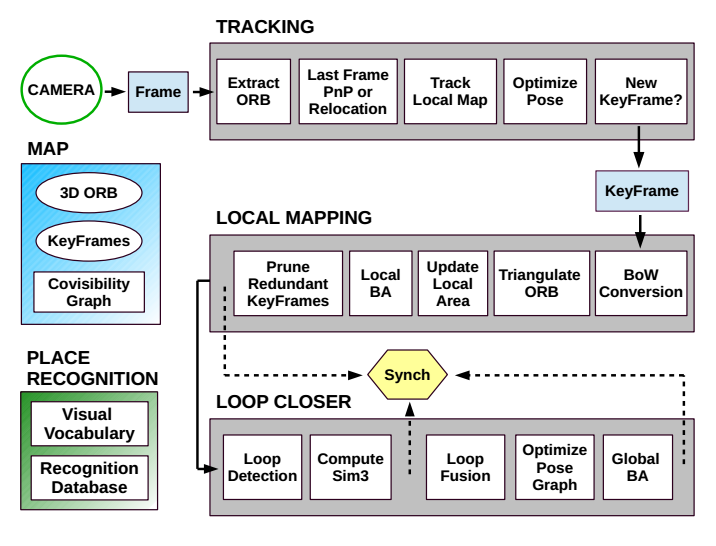
\includegraphics[scale=0.5]{figures/Fig3.6.png}
\caption{ORB-SLAM算法流程图}
\label{fig3.6}
\end{figure}

ORB-SLAM主要包括三个模块,特征跟踪,局部地图优化和闭环检测。特征跟踪模块负责提取新图像的特征点,并与临近的关键帧匹配估计当前帧的位姿并选择合适的图像作为新的关键帧;局部地图模块负责维护用于表示局部地图的Covisibility图,求解一个BA问题来优化局部地图中关键帧的位姿并筛选局部地图中的关键帧,剔除冗余;闭环检测模块对全局地图与关键帧进行回环检测,维护一个Pose图约束帧间位姿,消除累计误差。最后在每次闭环检测成功并优化结束后,独立进行一次全局BA,优化地图点位置,提高地图精度和一致性。


\subsubsection*{特征提取与匹配}
图像是由灰度和色彩组成的矩阵,如果直接从矩阵层面考虑运动估计会非常困难,基于特征的SLAM算法从图像中选取一些代表性的特征。为了保证在相机运动之后特征点保持稳定并可以在多个图像中找到,特征点应该满足如下性质
\begin{enumerate}[label={(\arabic*)}]
\item 可重复性:相同特征可以在不同的图像中被找到。
\item 可区别性:不同的特征有不同的表达。
\item 高效性:同一图像中,特征数量远小于像素数量。
\item 本地性:特征仅与小片图像区域相关。
\end{enumerate}

特征点由关键点和描数子两部分组成。关键点指该特征点在图像中的位置,有些特征点具有朝向、大小等信息;描述子通常由方向向量表示,按照人为设计的方式,描述该点周围像素的信息,描述子的设计原则是相似的特征应该有相似的描述子。因而,当两个特征的描述子在向量空间上的距离近似,可以人为是相同的特征。

ORB特征由关键点和描述子两部分组成。其关键点成为"Oriented FAST",FAST是一种图像角点,主要检测局部灰度变化明显的区域,提取速度块。ORB特征对原有的FAST特征点进行改进,添加了尺度和旋转不变性。旋转不变性通过构建尺度金字塔,并在金字塔每层检测角点来实现。旋转不变形则利用灰度质心法,以图像灰度值作为权重计算图像快质心,通过质心和几何中心设计方向向量保证特征旋转不变性;ORB特征的描述子为改进BRIEF描述子,BRIEF是一种二进制描述子,由0,1编码的向量表示关键点周围的两个像素的灰度大小关系。BRIEF使用随机选点的比较,速度快,存储方便,但是不具有旋转不变形。ORB特征在原有BRIEF描述子的基础上利用Oriented FAST关键点的方向信息,获取Steer BRIEF,使ORB特征描述子具有较好的尺度不变形。ORB特征相对于其他特征,如SHIFT、SURF特征,在保证精度和鲁棒性可用的前提下具有更好的计算速度和提取效率,适用于实时性要求较高的视觉SLAM算法。

\subsubsection*{数据关联与运动估计}
在完成图像特征提取后,需要对图像间的相同特征进行匹配。特征匹配是SLAM算法中重要的一部,解决SLAM算法的数据关联,确定了当前图像特征与之前图像特征的对应关系。考虑两个时刻的图像,如果图像$I_t$中提取的特征点$x_t^m,m=1,2,\cdots,M$,在图像$I_{t+1}$中提取到特征点$x_{t+1}^n,n=1,2,\cdots,N$,最简单的方法是进行暴力匹配,对每个特征点$x_t^m$与所有的特征点$x_{t+1}^n$测量描述子之间的距离,取最接近的作为匹配点。描述子距离表示描述子的相似程度,对于浮点类型的描述子可以使用欧氏距离,对于BRIEF这样的二进制描述子,一般使用汉明距——比较描述子不同位的个数。暴力匹配是最直接的方法,单当特征点数量较多,尤其与地图进行匹配时,暴力匹配将消耗很大的计算量,无法满足SLAM算法实时性要求。ORB-SLAM引入恒速模型匹配,假设当前帧的运动与上一帧相同从而得到初始位姿,之后利用出事位姿将上一帧或地图点投影到当前帧就近匹配,极大的提高了匹配速度。

当完成特征点匹配后,需要根据特征匹配关系估计相机运动。首先在初始化阶段,由于单目只知道2D像素坐标信息,需要根据对极几何解决初始位姿估计,对极几何描述了匹配特征点之间的几何关系,如图\ref{fig3.7}所示。
\begin{figure}[h]
% ch7 图7-7
\centering
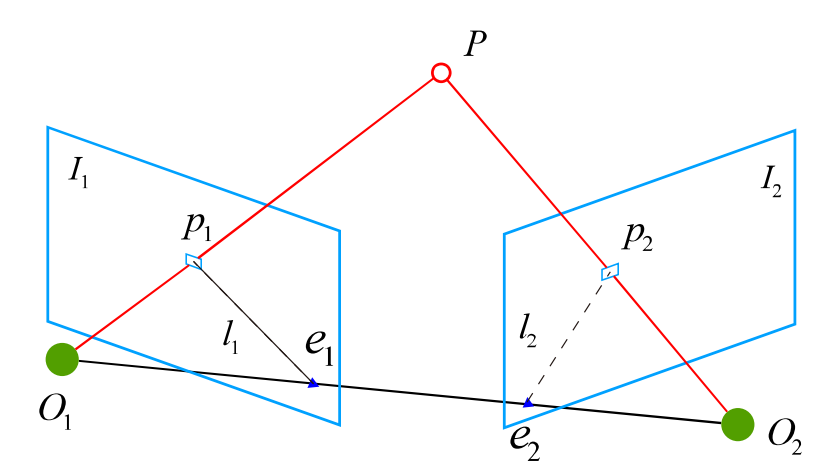
\includegraphics[scale=0.5]{figures/Fig3.7.png}
\caption{对极几何约束}
\label{fig3.7}
\end{figure}
假设第一帧到第二帧的相对运动为$\boldsymbol{R}$,$\boldsymbol{t}$,两个相机中心分别为$O_1$,$O_2$。考虑空间点$P=[X,Y,Z]^T$在两帧图像上的对应特征点$\boldsymbol{p}_1$,$\boldsymbol{p}_2$。根据相机投影模型,有
\begin{equation}
\label{equ3.15}
s_1 \boldsymbol{p}_1 = \boldsymbol{K} \boldsymbol{P}, \ \ \ 
s_2 \boldsymbol{p}_2 = \boldsymbol{K} (\boldsymbol{R} \boldsymbol{P}+\boldsymbol{t})
\end{equation}
在公式\eqref{equ3.15}中$\boldsymbol{K}$表示相机内参,$s_1$,$s_2$表示在两相机坐标系下的空间点深度,空间点坐标使用齐次坐标表示,现在取
\begin{equation}
\label{equ3.16}
\boldsymbol{x}_1 = \boldsymbol{K}^{-1} \boldsymbol{p}_1, \ \ \ 
\boldsymbol{x}_2 = \boldsymbol{K}^{-1} \boldsymbol{p}_2
\end{equation}
将方程\eqref{equ3.16}带入方程\eqref{equ3.15}中,可以得到
\begin{equation}
\label{equ3.17}
s_2 \boldsymbol{x}_2 = s_1 \boldsymbol{R} \boldsymbol{x}_1 + \boldsymbol{t}
\end{equation}
将方程\eqref{equ3.17}两侧同左乘$\boldsymbol{t}$的反对称矩阵$\boldsymbol{t}^{\wedge}$,再左乘$\boldsymbol{x}_2^T$,有
\begin{equation}
\label{equ3.18}
\boldsymbol{x}_2^T  \boldsymbol{t}^{\wedge}  \boldsymbol{R} \boldsymbol{x}_1 = \boldsymbol{x}_2^T \boldsymbol{t}^{\wedge} \boldsymbol{x}_2 = 0
\end{equation}
重新带入$\boldsymbol{p}_1$,$\boldsymbol{p}_2$可以得到
$\boldsymbol{x}_2^T$,有
\begin{equation}
\label{equ3.19}
\boldsymbol{p}_2^T \boldsymbol{K}^{-T} \boldsymbol{t}^{\wedge}  \boldsymbol{R} \boldsymbol{K}^{-1} \boldsymbol{p}_1  = 0
\end{equation}
公式\eqref{equ3.18}, \eqref{equ3.19}都称为对极约束,同时包含了旋转和平移信息。两方程中间的矩阵分别记为本质矩阵$\boldsymbol{E} = \boldsymbol{t}^{\wedge}  \boldsymbol{R} $和基本矩阵$\boldsymbol{F} = \boldsymbol{K}^{-T} \boldsymbol{t}^{\wedge}  \boldsymbol{R} \boldsymbol{K}^{-1}$。通过分解以两个矩阵,可以获得两帧图像之间的帧间相对运动。之后对估计运动的两帧关键帧的匹配特征进行三角化,得到出事地图点云的空间坐标。根据之前对极约束中的公式\eqref{equ3.17},同时左乘$\boldsymbol{x}_1^{\wedge}$可以得到
\begin{equation}
\label{equ3.20}
s_2 \boldsymbol{x}_1^{\wedge} \boldsymbol{R} \boldsymbol{x}_2 + \boldsymbol{x}_1^{\wedge} \boldsymbol{t} = s_1 \boldsymbol{x}_1^{\wedge} \boldsymbol{x}_1 = 0
\end{equation}
通过求解方程\eqref{equ3.20}可以直接得到$s_2$,根据求得结果可以很容易得到$s_1$。需要注意的是,由于单目无法提供深度信息,以上估计的位姿和地图点位置无法确定准确的尺度,一般将初始化地图点深度均值归一化为1。

在ORB-SLAM完成初始化得到初始关键帧和地图后,对于之后的帧图像,利用恒速模型提供给每帧图像位姿初值,将上一帧中的地图点投影到当前帧中,在阈值范围内搜索匹配点,通过最小化重投影误差求解当前帧的位姿。考虑$n$个三维空间点P和他们的投影p,当前帧的位姿$\boldsymbol{R}$,$\boldsymbol{t}$用李代数$\boldsymbol{\xi}$表示。假设空间点坐标为$P_i=[X_i,Y_i,Z_i]^T$,其投影的像素坐标为$\boldsymbol{u}_i = [u_i,v_i]T$,根据相机投影模型有
\begin{equation}
\label{equ3.21}
s_i
\begin{bmatrix}
u_i \cr v_i \cr 1\cr 
\end{bmatrix}
=
\boldsymbol{K} \exp\left( \boldsymbol{\xi}^{\wedge} \right)
\begin{bmatrix}
X_i \cr Y_i \cr Z_i \cr 1 \cr
\end{bmatrix}
\end{equation}
方程\eqref{equ3.21}表示根据位姿预测的空间点投影像素位置,由于相机位姿存在误差且系统存在观测误差,观测到的匹配点$p_i$与预测值存在误差,可以构建BA问题优化相机位姿,优化函数为。
\begin{equation}
\label{equ3.22}
\boldsymbol{\xi}^* = \argmin\limits_{\boldsymbol{\xi}} {1 \over 2} \sum\limits_{i=1}^n  \left \Vert \boldsymbol{p}_i - {1 \over s_i} \boldsymbol{K} \exp\left( \boldsymbol{\xi}^{\wedge} \right) \boldsymbol{P}_i  \right \Vert_2^2
\end{equation}
方程\eqref{equ3.22}中的误差称为重投影误差,利用李代数可以构建无约束优化问题,通过高斯-牛顿(G-N)或列文伯格-马夸尔特方法(L-M)等优化方法可以很容易的求解。

%3.3
\section{两种SLAM算法比较}
之前的内容主要针对主流的单目SLAM算法原理进行了分析,本节将在具体数据集上对两个主流的SLAM算法基于直接法的LSD-SLAM和基于特征的ORB-SLAM算法进行实验和比较,对比两种算法的定位精度、鲁棒性和地图重建效果,根据实验结果分析两种SLAM算法的优缺点。结合无人机飞行器的运动特性选择合适的视觉SLAM定位方法,并针对其存在的问题提出改进方案。

\subsubsection*{定位精度}
TUM RGB-D数据集包含了多种室内场景的图像序列,并且每个序列通过外部视觉捕捉系统提供了准确的真实轨迹,适用于评估视觉SLAM系统的定位精度。对单目SLAM算法进行实验测试时,只使用TUM数据集的RGB图像。对于单目SLAM输出的轨迹结果,通过$\mathfrak{sim}(3)$相似变换进行轨迹对齐,比较关键帧的绝对轨迹误差的均方根误差(RMSE),误差表示为:
\begin{equation}
\label{equ3.23}
\begin{aligned}
\boldsymbol{F}_i &\doteq \boldsymbol{Q}_i^{-1} S \boldsymbol{P}_i
\\ 
R\!M\!S\!E(\boldsymbol{F}) &\doteq \left( {1 \over n} \sum\limits_{i=1}^n \left \Vert trans(\boldsymbol{F}_i) \right \Vert^2 \right)^{1 \over 2} 
\end{aligned}
\end{equation}
其中$\boldsymbol{Q}_i$表示真值轨迹第$i$时刻的位置,$\boldsymbol{P}_i$表示估计轨迹第$i$时刻的位置,$\boldsymbol{S}$表示用于对齐估计的$\mathfrak{sim}(3)$相似变换,结果如下表\ref{tab3.1}所示
\begin{table}[h]		%表格环境
% \multicolumn是跨列功能,第一个参数2,表示跨两列,第二个参数c|,表示文字置中,并在栏位右边画一条直线框,最后一个参数即是要填入的文字
%\multirow是跨行功能,第一个参数2,表示跨两行,第二个参数*,表示系统自动调整文字,最后一个参数即是要填入的文字
\newcommand{\tabincell}[2]{\begin{tabular}{@{}#1@{}}#2\end{tabular}}		%单元格内容强制换行
\renewcommand\arraystretch{1.5}		%增加行间距
\centering
\caption{TUM数据集单目SLAM算法定位精度}   % 表格标题,在表格内容之前
\label{tab3.1}
	\begin{tabular*}{0.9\textwidth}{@{\extracolsep{\fill}}ccc}  %生成行和列的表格
	%\begin{tabular}{p{2cm}p{1.5cm}p{1.5cm}p{1.5cm}}	
	
	\toprule
	
	\multicolumn{1}{c}{\multirow{2}{*}{Seq.}} &
	\multicolumn{2} {c} {\bfseries\tabincell{c} {Absolute Key Frame Trajectory RMSE(cm)}} \\
	\cline{2-3}								%在上一行下面,2-4列画横线
	\multicolumn{1}{c}{}&
	\multicolumn{1}{c}{LSD SLAM}	&
	\multicolumn{1}{c}{ORB SLAM}	\\	
	
	\midrule
	
	\multicolumn{1}{c}{fr1/xyz}		&
	\multicolumn{1}{c}{0.90}		&
	\multicolumn{1}{c}{9.00}		\\
	
	\multicolumn{1}{c}{fr2/xyz}		&
	\multicolumn{1}{c}{0.30}		&
	\multicolumn{1}{c}{2.15}		\\
	
	\multicolumn{1}{c}{fr1/desk}	&
	\multicolumn{1}{c}{1.69}		&
	\multicolumn{1}{c}{10.65}		\\
	
	\multicolumn{1}{c}{fr2/desk}	&
	\multicolumn{1}{c}{0.88}		&
	\multicolumn{1}{c}{4.57}		\\
	
	\multicolumn{1}{c}{fr2/desk\_ person}	&
	\multicolumn{1}{c}{0.63}		&
	\multicolumn{1}{c}{31.73}		\\
	
	\multicolumn{1}{c}{fr3/long\_ office}	&
	\multicolumn{1}{c}{3.45}		&
	\multicolumn{1}{c}{38.53}		\\

	\multicolumn{1}{c}{fr3/sit\_ xyz}	&
	\multicolumn{1}{c}{0.79}		&
	\multicolumn{1}{c}{7.73}		\\	
	
	\multicolumn{1}{c}{fr3/walk\_ halfsph}	&
	\multicolumn{1}{c}{1.74}		&
	\multicolumn{1}{c}{$\boldsymbol{X}$}		\\	
	\bottomrule
	
	\end{tabular*}
\end{table}
表\ref{tab3.1}是在数据集连续测试五次取均值的结果,符号$\boldsymbol{X}$表示运行过程中出现丢失无法完成整个数据集。通过表\ref{tab3.1}可以看出,ORB-SLAM算法的定位精度高于LSD-SLAM,对于存在运动目标的场景具有较好的定位精度。主要原因可能是:(1)基于直接法的LSD-SLAM算法遵从灰度不变假设,对于相机内参和曝光非常敏感,而且直接法SLAM在相机运动过快时无法准确估计位姿;而基于特征的SLAM算法使用特征提取与匹配的方法关联和解算位姿,对传感器参数变化较为鲁棒,并且在快速运动时不易丢失。(2)基于直接法的SLAM算法计算复杂度较大,无法多次优化关键帧位姿并且将关键帧位姿与地图点的联合BA优化简化为pose图优化,影响了定位精度。另外,由于单目无法提供深度信息,因而估计的轨迹缺少尺度信息。

\subsubsection*{地图重建效果}
选择TUM数据集中具有代表性的fr2/xyz,fr2/desk,fr3/long\_ office数据集对比重构效果,重构效果如下图所示
\begin{figure}[h]
\centering
	\subfigure[LSD-SLAM]
    {
		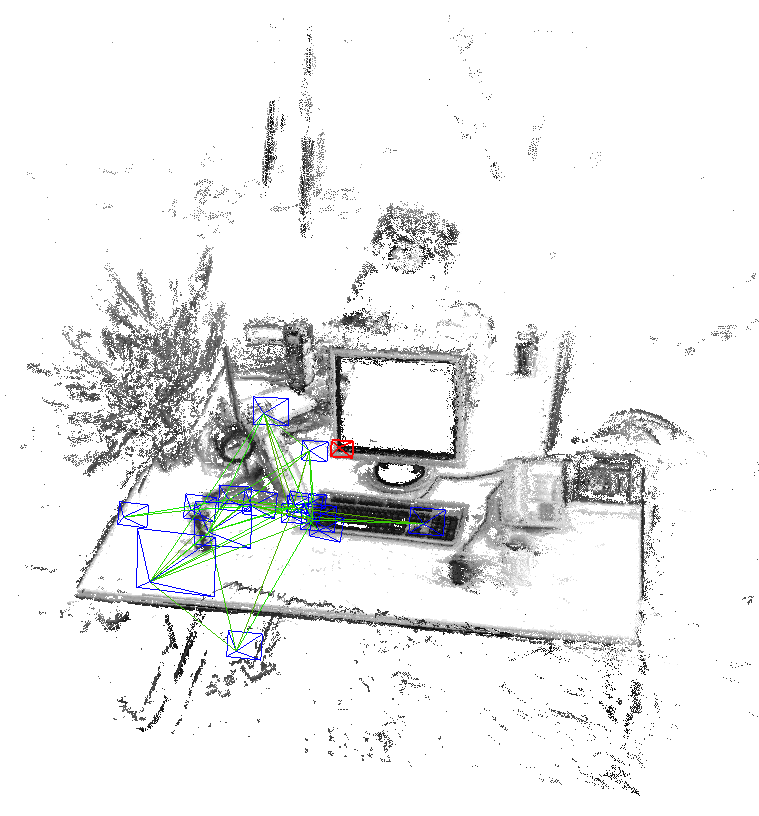
\includegraphics[scale=.24]{figures/Fig3.8_a.png}
	}
	\subfigure[ORB-SLAM]
    {	
		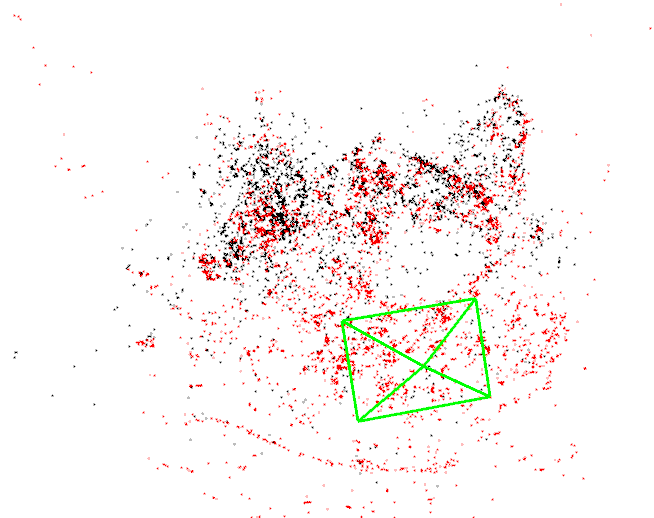
\includegraphics[scale=.3]{figures/Fig3.8_b.png}
	}
\caption{fr2/xyz场景}
\label{fig3.8}
\end{figure}

\begin{figure}[h]
\centering
	\subfigure[LSD-SLAM]
    {
		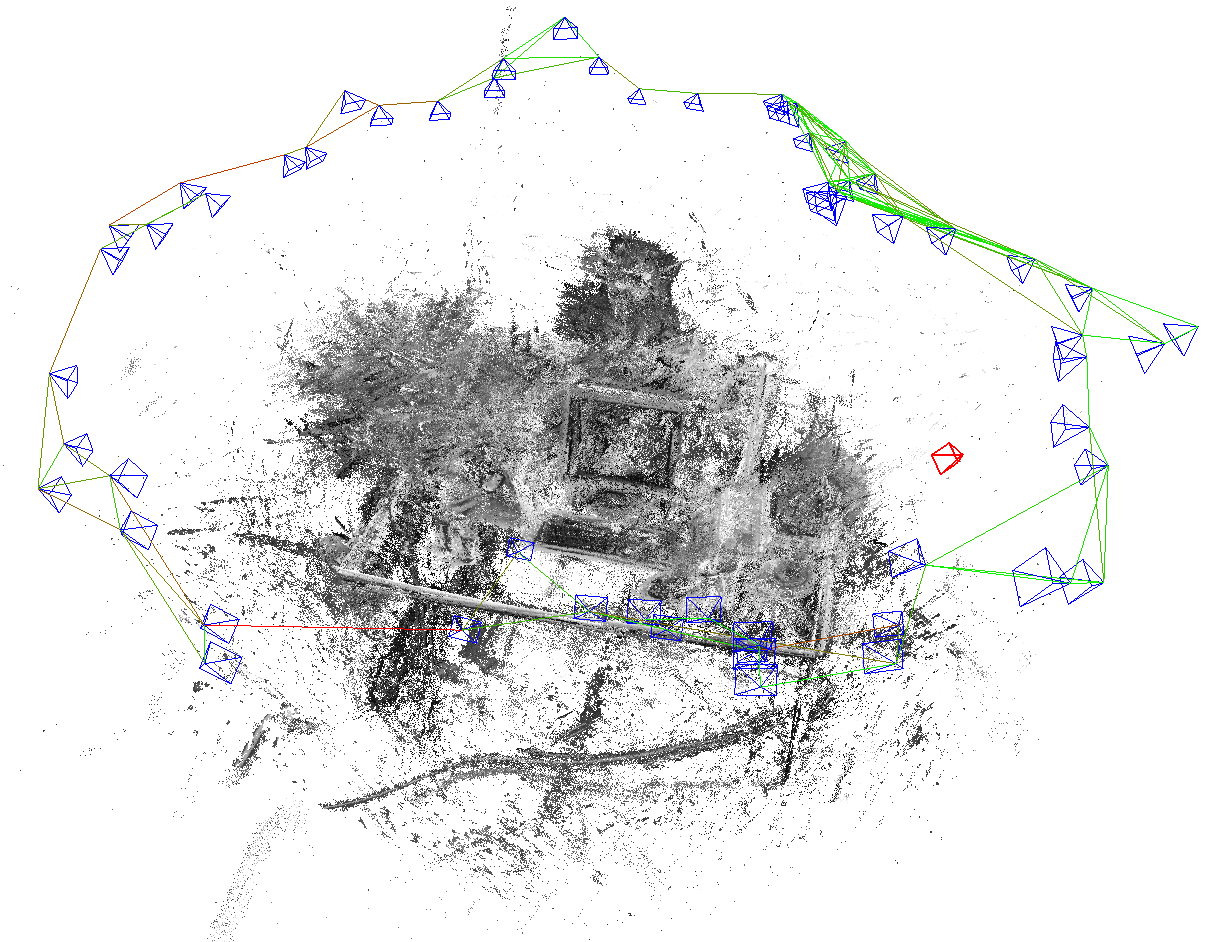
\includegraphics[scale=.15]{figures/Fig3.9_a.png}
	}
	\subfigure[ORB-SLAM]
    {	
		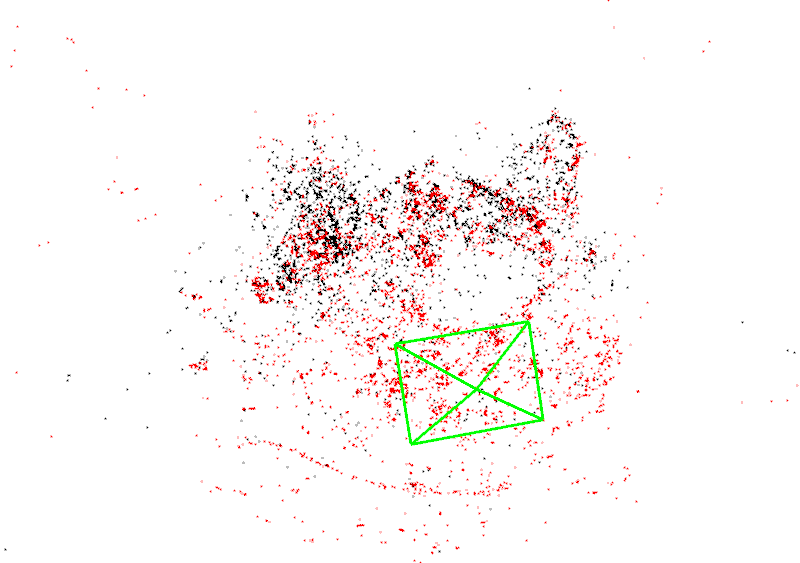
\includegraphics[scale=.3]{figures/Fig3.9_b.png}
	}
\caption{fr2/desk场景}
\label{fig3.9}
\end{figure}

\begin{figure}[h]
\centering
	\subfigure[LSD-SLAM]
    {
		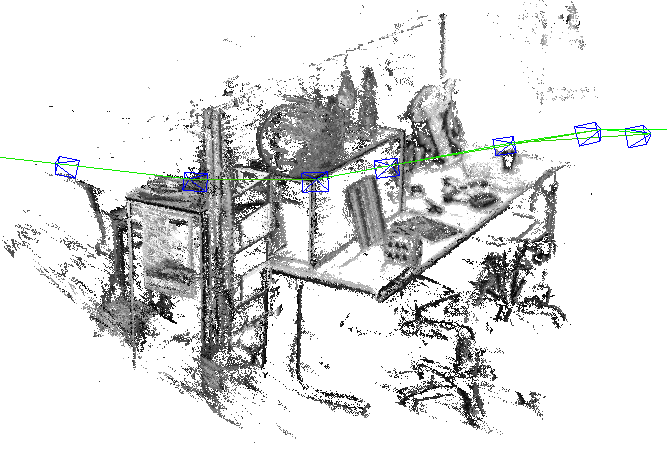
\includegraphics[scale=.25]{figures/Fig3.10_a.png}
	}
	\subfigure[ORB-SLAM]
    {	
		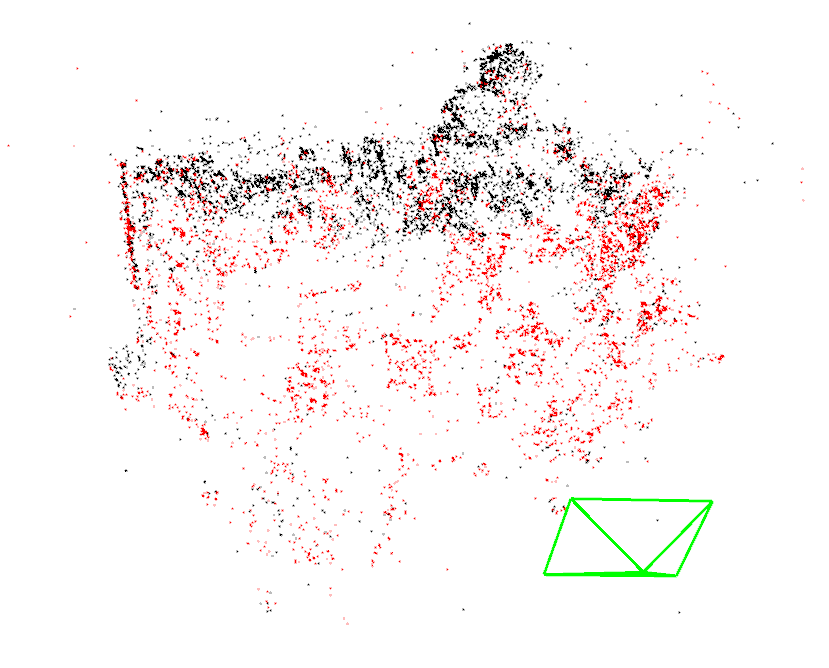
\includegraphics[scale=.21]{figures/Fig3.10_b.png}
	}
\caption{fr3/long\_ office场景}
\label{fig3.10}
\end{figure}

通过对比以上重建结果可以看出,基于直接法的LSD-SLAM算法可以恢复环境的半稠密地图,通过地图可以进行目标识别,导航与任务规划等其他任务;而基于特征的ORB-SLAM算法只能恢复环境稀疏的点云地图,无法提供更多的环境信息。造成这样结果的原因在于,基于特征的SLAM算法只恢复环境的特征点对应的地图点云,考虑特征点的性质:其数量远低于像素数量,因而无法提供丰富的环境场景信息。直接法SLAM关联灰度变化明显区域的像素,而灰度变化明显的像素一般为物体边缘,因而可以恢复出环境的半稠密地图。

%3.4
\section{本章小结}
本章介绍了单目视觉SLAM的结构框架、算法原理和分类,从实现原理,定位精度,鲁棒性和地图重建效果4个方面比较了经典的基于直接法的LSD-SLAM算法和基于特征的ORB-SLAM算法。结果表明,相比于基于直接法的LSD-SLAM算法,基于特征的ORB-SLAM算法具有较好的光度不变性和视角不变性,可以在宽基线条件下稳定匹配,对于快速运动鲁棒性好,适宜作为无人机的感知定位系统。但也存在两个问题,首先基于特征的ORB-SLAM算法重建地图为稀疏点云地图,环境信息较少,无法用于无人机的导航、避障与路径规划;另外,由于单目相机无法提供环境尺度,因而估计得到的轨迹尺度不确定。针对ORB-SLAM算法存在的问题,在第四章研究基于特征的SLAM算法的半稠密重建,提供丰富的环境信息;在第五章研究基于IMU-视觉融合的惯性视觉单目SLAM算法,解决单目SLAM算法的尺度问题。通过以上改进,使得本文研究的单目SLAM算法具有准确的尺度,较好的定位精度和丰富的环境信息,为无人机提供准确的位姿估计和环境信息。




\iffalse
\begin{table}
\newcommand{\tabincell}[2]{\begin{tabular}{@{}#1@{}}#2\end{tabular}}		%单元格内容强制换行
\centering
\caption{TUM数据集下单目SLAM算法定位精度}	% NOTE!  caption goes _before_ the table contents !!
\renewcommand\arraystretch{1.5}		%增加行间距
%\begin{small}							%控制字体大小
\begin{tabular}{p{2cm}p{1.5cm}p{1.5cm}p{1.5cm}}
%\hline									%  结束的那一行画一根水平的直线
\toprule
% \multicolumn是跨列功能,第一个参数2,表示跨1列,第二个参数c|,表示文字置中,并 在栏位右边画一条直线框,最后一个参数即是要填入的文字
\multicolumn{1}{c}{\multirow{3}{*}{Seq.}} & 
\multicolumn{2} {c} {\bfseries\tabincell{c} {Absolute Key Frame Trajectory RMSE(cm)}} \\
\cline{2-3}								%在上一行下面,2-4列画横线
\multicolumn{1}{c}{}&   
\multicolumn{1}{c}{\bfseries \tabincell{c}{LSD-SLAM} } &     
\multicolumn{1}{c}{\bfseries \tabincell{c}{ semi-dense \\mono-VO}}  \\
%\multicolumn{1}{c}{\bfseries \tabincell{c}{ RGB-D \\SLAM}} \\	
%\cline{1-3}
\midrule
\multicolumn{1}{c}{fr2/desk}	&
\multicolumn{1}{c}{5.65}		&
\multicolumn{1}{c}{13.50}      \\
%\multicolumn{1}{c}{2.58}   \\

\multicolumn{1}{c}{Fr2/xyz}  &
\multicolumn{1}{c}{2.15}     &
\multicolumn{1}{c}{3.79}      \\
%\multicolumn{1}{c}{1.34}    \\

\multicolumn{1}{c}{sim/slowmo}  &
\multicolumn{1}{c}{0.37}        &
\multicolumn{1}{c}{2.21}        \\
%\multicolumn{1}{c}{0.13}        \\
%\hline
\bottomrule
\end{tabular}
%\end{small}	
\end{table}
\fi




\iffalse
The current frames will replace the current key frames according with the Direct SE(3) image alignment. An existing key frame ${k_i} = ({I_i},{D_i},{V_i})$, the relative posture ${\xi _{ji}} \in se(3)$ of a new image ${I_j}$ is obtained by minimizing the variance-normalized photometric error

\begin{equation}
E_{p}(\xi _{ji}) = \sum\limits_{p \in \Omega _{D_{i}}} \left\|  \frac{r_{p}^{2} (p,\xi_{ji})}{\sigma_{r_{p}}^{2} (p,\xi_{ji})}  \right\|_{\delta}
\end{equation}


\begin{equation}
r_{p}(p,\xi _{ji}): = I_{i}(p) - I_{j}(\omega (p,D_{i}(p),\xi _{ji}))
\end{equation}

\begin{equation}
\sigma _{r_{p}} ^{2}(p,\xi _{ji}): = 2\sigma _{I} ^{2} + {\left( \frac {\partial r_{p}(p,\xi_{ji})} {\partial D_{i} (p)} \right)^{2}} V_{i}(p)
\end{equation}

The formula (13) is the Huber norm and applied to the normalized residual.

\begin{equation}
{\left\| r^{2} \right\|_{\delta}}:=\left\{\begin{array}{ll}
\frac {r^{2}} {2\delta}            & |r|\leq \delta       \\
|r|-\frac {\delta} {2}      & |r| > \delta
\end{array} \right.
\end{equation}




If the camera moves too far away from the existing map, a new key frame is created from the most recent tracked image. We threshold a weighted combination of relative distance and angle to the current key frame

\begin{equation}
dist({\xi _{ji}}): = \xi _{ji}^TW{\xi _{ji}}
\end{equation}

Where W is a diagonal matrix containing the weights. Note that, as described in the following section, each key frame is scaled such that its mean inverse depth is one. This threshold is therefore relative to the current scale of the scene, and ensures sufficient possibilities for small-baseline stereo comparisons.

Once a new frame is chosen to become a key frame, its depth map is initialized by projecting points from the previous key frame into it, followed by one iteration of spatial regularization and outlier removal [5]. Afterwards, the depth map is scaled to have a mean inverse depth of one -this scaling factor is directly incorporated into the sim(3) camera pose. Finally, it replaces the previous key frame and is used for tracking subsequent new frames.

In contrast to RGB-D or Stereo SLAM, monocular SLAM is inherently scale-ambivalent, the absolute scale of the world is not observable. Over long trajectories this leads to scale-drift, which is one of the major sources of error [9]. Further, all distances are only defined up to scale, which causes threshold-based outlier rejection or parametrized robust kernels to be ill-defined.

We select an advanced method in [1] for better perform direct, scale-drift image alignment, which is used to align two differently scaled key frames. For the photometric residual ${r_p}$, the depth residual ${r_d}$ which penalizes deviations in inverse depth between key frames, allowing to directly estimate the scaled transformation between them. The total error function becomes

\begin{equation}
E({\xi _{ji}}): = {\sum\limits_{p \in {\Omega _{{D_i}}}} {\left\| {\frac{{r_p^2(p,{\xi _{ji}})}}{{\sigma _{{r_p}(p,{\xi _{ji}})}^2}} + \frac{{r_d^2(p,{\xi _{ji}})}}{{\sigma _{{r_d}(p,{\xi _{ji}})}^2}}} \right\|} _\delta }
\end{equation}
the depth residual is computed

\begin{equation}
r_{d}(p,\xi _{ji}): = [p^{'}]_{3} - D_{j}([p^{'}]_{1,2})
\end{equation}

% 公式换行用 \\ 
\begin{equation}
\begin{split}
\sigma_{r_{d}(p,\xi_{ji})} ^{2} :=V_{j}( [ p^{'} ]_{1,2} )  {\left( \frac {\partial r_{d}(p,\xi_{ji})} {\partial D_{j} \left[ p^{'} \right]_{1,2}}  \right)^{2}} + V_{i}(p) \left( \frac {\partial r_{d}(p,\xi_{ji})} {\partial D_{j}(p)} \right)
\end{split}
\end{equation}

After a new key frame ${k_i}$ is added to the map, a number of possible loop closure key frames ${k_{ji}},....{k_{jn}}$ is collected. We use the closet ten key frames, as well as a suitable candidate. To avoid insertion of false or falsely tracked loop closures, we then perform a reciprocal tracking check. For each candidate ${k_{jk}}$ we independently track ${\xi _{{j_k}i}}$ and ${\xi _{i{j_k}}}$.

\begin{equation}
e\!(\!{\xi _{{j_k}i}},{\xi _{i{j_k}}})\!: \!= \!{\!(\!{\xi _{{j_k}i}} \!\circ \!{\xi _{i{j_k}}})\!^T}{\!(\!{\Sigma _{{j_k}i}}\! +\! Ad{j_{{j_k}i}}{\Sigma _{i{j_k}}}Adj_{{j_k}i}^T\!)\!^{ - 1}}\!(\!{\xi _{{j_k}i}}\! \circ\! {\xi _{i{j_k}}}\!)
\end{equation}

Only if the two estimates are statistically similar, if formula (18) is sufficiently small, they are added to the global map. For this, the adjoint $Ad{j_{{j_k}i}}$ is used to transform ${\Sigma _{i{j_k}}}$ into the correct tangent space.

The map is represented as a pose graph of keyframes: Each keyframe $\kappa_{i}$ consists of a camera image $I_{i}\!:\!\Omega_{D_{i}}\!\rightarrow \!{\mathbb{R}}$,an inverse depth map $D_{i}\!:\!\Omega_{D_{i}}\!\rightarrow \!{\mathbb{R}}^{+}$, and the variance of the inverse depth $ V_{i}\!:\!\Omega_{D_{i}}\!\rightarrow \!{\mathbb{R}}^{+}$.Note that the depth map and variance are only defined for a subset of pixels $ \Omega_{D_{i}}\!\subset\!\Omega_{i} $, containing all image regions in the vicinity of sufficiently large intensity gradient, hence semi-dense.Edges $ \varepsilon_{ji}$ between keyframes contain their relative alignment as similarity transform $ \xi_{ji}\in sim(3) $, as well as the corresponding covariance matrix $\Sigma_{ji} $

The map, consisting of a set of keyframes and tracked sim(3)-constraints, is continuously optimized in the background using pose graph optimization. The
error function that is minimized is in accordance with the left-multiplication convention
\begin{equation}
E(\xi\!_{W\!_{1}}\!...\!\xi\!_{W\!_{n}})\!:\!= \sum\limits_{(\!\xi\!_{ji},\Sigma\!_{ji}\!)\!\in\!\varepsilon}\!(\!\xi_{ji}\!\circ\!\xi_{\!W_{i}\!}^{-1}\! \!\circ\!\xi_{\!W\!_{j}}\!)\!^{T}\!\Sigma_{\!j\!i}^{\!-1\!}\!(\!\xi_{ji}\!\circ\!\xi_{\!W_{i}\!}^{-1}\! \!\circ\!\xi_{\!W\!_{j}}\!)
\end{equation}
\fi
